\section{Computing Gradients of Tensor Networks}\label{chapter:gradients}
Optimizing tensor networks in a general setting is a significant challenge in many research areas. Although many optimization techniques have been developed for matrices, extending these methods to tensor networks can remain challenging~\citep{liao2019differentiable}. This complexity stems from the high computational cost of tensor contractions and the lack of efficient optimization algorithms for higher-dimensional cases. Additionally, manually computing gradients using the chain rule can seem daunting beyond simple tensor network structures. In this chapter, we introduce an elegant and intuitive approach for deriving higher-order derivatives using the graphical notation of a tensor network. This approach illustrates that derivatives of tensor network functions often inherit the low-rank structure of the initial tensor network.

In the next section, we first define the classical concepts of gradient and Jacobian for functions that take vectors as input. We then extend these concepts to functions that take tensors as inputs and produce tensors as outputs.
\subsection{Jacobians}
We first recall the classical notions of gradient and Jacobian of functions defined over $\mathbb{R}^n$.

\begin{definition}
  For $f:\RR^n\to\RR$ and $g:\RR^n\to\RR^p$. The gradient of $f$ and the Jacobian of $g$ at $\theta\in\mathbb{R}^n$ are defined by
    $$\nabla_\theta f = \left[\frac{\partial f(\theta)}
{\partial\theta_1},\frac{\partial f(\theta)}{\partial\theta_2},\dots,\frac{\partial f(\theta)} 
    {\partial\theta_n}\right]^\ts
        =
    \begin{tikzpicture}[baseline=\baseline]
    \tikzset{tensor/.style = {minimum size = 0.5cm,shape = circle,thick,draw=black,inner sep = 0pt}, edge/.style   = {thick,line width=.4mm}}
    \def\y{0}
     \def\x{0}
    \node[tensor,fill=blue!40!red!60!white] (a1) at (\x,\y){};
    \draw[edge](a1) -- (\x+0.75,\y)node [midway, above]{\edgelabel{$n$}};
    \end{tikzpicture} \in\mathbb{R}^n,$$
    and 
    $$\frac{\partial g(\theta)}{\partial\theta} = \left(\frac{\partial g(\theta)_i}{\partial\theta_j}\right)_{i=1,\cdots,p\atop j=1,\cdots, n}
    =
    \begin{tikzpicture}[baseline=\baseline]
    \tikzset{tensor/.style = {minimum size = 0.5cm,shape = circle,thick,draw=black,inner sep = 0pt}, edge/.style   = {thick,line width=.4mm}}
    \def\y{0}
     \def\x{0}
    \node[tensor,fill=blue!20!red!50!white] (A) at (\x,\y){};
    \draw[edge](A) -- (\x+0.75,\y)node [midway, above]{\scalebox{0.7}{\dimcolor{$n$}}};
    \draw[edge](A) -- (\x-0.75,\y)node [midway, above]{\scalebox{0.7}{\dimcolor{$p$}}};
    \end{tikzpicture}\in\mathbb{R}^{p\times n}.$$  
\end{definition}
We can naturally extend the notion of Jacobian to functions that take tensors as input and output tensors~(of arbitrary orders).

\begin{definition}
 Let $f:\RR^{n_1\times\dots\times n_N}\to\RR^{m_1\times\dots\times m_M}$,. The \emph{Jacobian tensor} of $f$ at $\theta\in\RR^{n_1\times\dots\times n_N}$ is the tensor $\frac{\partial f}{\partial\theta}\in\RR^{m_1\times\dots\times m_M\times n_1\times\dots\times n_N}$
 defined by
\begin{align*}
   \frac{\partial f(\theta)}{\partial\theta} 
   &= 
   \left(\frac{\partial f(\theta)_{i_1,\dots,i_M}}{\partial\theta_{j_1,\dots,j_N}}\right)_{i_1\in[m_1],\cdots,i_M\in[m_M]\atop j_1\in[n_1],\cdots,j_N
\in[n_N]}\\
&=
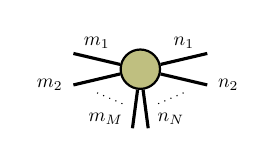
\begin{tikzpicture}[baseline=-0.5ex]
    \tikzset{tensor/.style = {minimum size = 0.5cm,shape = circle,thick,draw=black,inner sep = 0pt}, edge/.style = {thick,line width=.4mm},every loop/.style={}}
    \def\x{6}
    \node[tensor,fill=green!50!red!50!white] (T) at (\x,0) {};
    \draw[edge] (T) -- (\x-0.85,0.2)node [midway, above]{\scalebox{0.7}{\dimcolor{$m_1$}}};
    \draw[edge] (T) -- (\x-0.85,-0.2)node [left]{\scalebox{0.7}{\dimcolor{$m_2$}}};
    \draw[edge] (T) -- (\x-0.1,-0.75)node [near end, left]{\scalebox{0.7}{\dimcolor{$m_M$}}};
    \draw[dotted] (\x-0.55,-0.3) -- (\x-0.2,-0.45);
    \draw[edge] (T) -- (\x+0.85,0.2)node [midway, above]{\scalebox{0.7}{\dimcolor{$n_1$}}};
    \draw[edge] (T) -- (\x+0.85,-0.2)node [right]{\scalebox{0.7}{\dimcolor{$n_2$}}};
    \draw[edge] (T) -- (\x+0.1,-0.75)node [near end, right]{\scalebox{0.7}{\dimcolor{$n_N$}}};
    \draw[dotted] (\x+0.55,-0.3) -- (\x+0.2,-0.45);
    \end{tikzpicture}\in\RR^{m_1\times\cdots\times m_M\times n_1\times\cdots\times n_N}. 
\end{align*}
\end{definition}




The following theorem demonstrates that first-order derivatives of tensor networks with respect to a core tensor can be easily computed using tensor networks.

\begin{theorem}\label{thm:gradients}
    Let $\Tt$ be a tensor given as a tensor network, where $\Gt$ is a core tensor \emph{appearing only once} in the tensor network. Then $\frac{\partial \Tt}{\partial \Gt}$ is obtained by removing $\Gt$ from the tensor network of $\Tt$. 
\end{theorem}
The following examples illustrate how Theorem~\ref{thm:gradients} can be applied to tensor networks.
\paragraph{Examples}
Let 
$\begin{tikzpicture}[baseline=\baseline]
    \tikzset{tensor/.style = {minimum size = 0.5cm,shape = circle,thick,draw=black,inner sep = 0pt}, edge/.style = {thick,line width=.4mm},every loop/.style={}}
    \def\x{0}
    \def\y{0}
     \node[tensor,fill=green!50!red!50!white] (B) at (\x+1,\y) {$\Xt$};
    \draw[edge] (B) -- (\x+0.25,0) node [midway,above] {\scalebox{0.7}{\dimcolor{$d_1$}}};
    \draw[edge] (B) -- (\x+1.85,\y) node [midway,above] {\scalebox{0.7}{\dimcolor{$d_3$}}};
    \draw[edge] (B) -- (\x+1,\y-0.85) node [midway,left] {\scalebox{0.7}{\dimcolor{$d_2$}}};
\end{tikzpicture}
=
\begin{tikzpicture}[baseline=\baseline]
    \tikzset{tensor/.style = {minimum size = 0.5cm,shape = circle,thick,draw=black,inner sep = 0pt}, edge/.style = {thick,line width=.4mm},every loop/.style={}}
    \def\x{0}
    \def\y{0}
    \node[tensor,fill=red!30!white] (A) at (\x+2,\y) {$\Gt_1$};
    \node[tensor,fill=red!50!white] (B) at (\x+3.2,\y) {$\Gt_2$};
    \node[tensor,fill=blue!30!white] (C) at (\x+2.6,\y-0.7) {$\Gt_3$};
    \node[tensor,fill=blue!50!white] (D) at (\x+4.3,\y) {$\Gt_4$};
    \draw[edge] (A) -- (B) node [midway,above] {\scalebox{0.7}{\dimcolor{$R_1$}}};
    \draw[edge] (A) -- (C);
    \node[draw=none] () at (\x+2,\y-0.5) {\scalebox{0.7}{\dimcolor{$R_2$}}};
    \draw[edge] (B) -- (C);
    \node[draw=none] () at (\x+3.2,\y-0.5) {\scalebox{0.7}{\dimcolor{$R_3$}}};
    \draw[edge] (B) -- (D) node [midway,above] {\scalebox{0.7}{\dimcolor{$R_4$}}};
    \draw[edge] (A) -- (\x+2,\y+0.7) node [midway,left] {\scalebox{0.7}{\dimcolor{$d_1$}}};
    \draw[edge] (D) -- (\x+4.3,\y+0.7) node [midway,right] {\scalebox{0.7}{\dimcolor{$d_3$}}};
    \draw[edge] (C) -- (\x+2.6,\y-1.5) node [midway,left] {\scalebox{0.7}{\dimcolor{$d_2$}}};
\end{tikzpicture}
$ be a tensor network. Observe that we can think of $\Xt$ as a function of any of the core tensors of its tensor network representation. We can thus naturally ask what the Jacobian of $\Xt$ is with respect to, e.g., $\Gt_2$ or $\Gt_4$.
The previous theorem gives us an easy way to compute these derivatives:
\begin{itemize}
\item According to Theorem~\ref{thm:gradients}, to find the gradient of $\Xt$ with respect to $\Gt_2$, we need to remove the core $\Gt_2$ from the tensor network, i.e.,
$$
\frac{\partial}{\partial\Gt_2}\left(\begin{tikzpicture}[baseline=\baseline]
    \tikzset{tensor/.style = {minimum size = 0.5cm,shape = circle,thick,draw=black,inner sep = 0pt}, edge/.style = {thick,line width=.4mm},every loop/.style={}}
    \def\y{0}
    \def\x{0}
    \node[tensor,fill=red!30!white] (A) at (\x+2,\y) {$\Gt_1$};
    \node[tensor,fill=red!50!white] (B) at (\x+3.2,\y) {$\Gt_2$};
    \node[tensor,fill=blue!30!white] (C) at (\x+2.6,\y-0.7) {$\Gt_3$};
    \node[tensor,fill=blue!50!white] (D) at (\x+4.3,\y) {$\Gt_4$};
    \draw[edge] (A) -- (B) node [midway,above] {\scalebox{0.7}{\dimcolor{$R_1$}}};
    \draw[edge] (A) -- (C);
    \node[draw=none] () at (\x+2,\y-0.5) {\scalebox{0.7}{\dimcolor{$R_2$}}};
    \draw[edge] (B) -- (C);
    \node[draw=none] () at (\x+3.2,\y-0.5) {\scalebox{0.7}{\dimcolor{$R_3$}}};
    \draw[edge] (B) -- (D) node [midway,above] {\scalebox{0.7}{\dimcolor{$R_4$}}};
    \draw[edge] (A) -- (\x+2,\y+0.7) node [midway,left] {\scalebox{0.7}{\dimcolor{$d_1$}}};
    \draw[edge] (D) -- (\x+4.3,\y+0.7) node [midway,right] {\scalebox{0.7}{\dimcolor{$d_3$}}};
    \draw[edge] (C) -- (\x+2.6,\y-1.5) node [midway,left] {\scalebox{0.7}{\dimcolor{$d_2$}}};
    \end{tikzpicture}\right)
=
    \begin{tikzpicture}[baseline=\baseline]
    \tikzset{tensor/.style = {minimum size = 0.5cm,shape = circle,thick,draw=black,inner sep = 0pt}, edge/.style = {thick,line width=.4mm},every loop/.style={}}
    \def\y{-0.5}
    \def\x{0}
    \node[tensor,fill=red!30!white] (A) at (\x,\y+1) {$\Gt_1$};
    \node[tensor,fill=blue!30!white] (C) at (\x+0.6,\y+0.2) {$\Gt_3$};
    \node[tensor,fill=blue!50!white] (D) at (\x+2,\y+0.5) {$\Gt_4$};
    \draw[edge] (A) -- (C);
    \draw[edge] (A) -- (\x,\y+1.7) node [midway,left] {\scalebox{0.7}{\dimcolor{$d_1$}}};
    \draw[edge] (A) -- (\x+0.7,\y+1) node [midway,above] 
{\scalebox{0.7}{\dimcolor{$R_1$}}};
    \draw[edge] (D) -- (\x+3,\y+0.5) node [midway,above] {\scalebox{0.7}{\dimcolor{$R_4$}}};
    \draw[edge] (C) -- (\x+0.6,\y-0.7) node [midway,left] {\scalebox{0.7}{\dimcolor{$d_2$}}};
    \draw[edge] (C) -- (\x+1.3,\y+0.2) node [midway,above] {\scalebox{0.7}{\dimcolor{$R_3$}}};
    \draw[edge] (D) -- (\x+2,\y+1.3) node [midway,left] {\scalebox{0.7}{\dimcolor{$d_3$}}};
    \node[draw=none] () at (\x,\y+0.4) {\scalebox{0.7}{\dimcolor{$R_2$}}};
\end{tikzpicture}.
$$ 
To understand why this procedure works, we can view the tensor decomposition of $\Xt$ as a matrix-vector product:
$$
\Mb\vb 
=
\begin{tikzpicture}[baseline=\baseline]
    \tikzset{tensor/.style = {minimum size = 0.5cm,shape = circle,thick,draw=black,inner sep = 0pt}, edge/.style = {thick,line width=.4mm},every loop/.style={}}
    \def\y{1}
    \def\x{0}
     \node[tensor,fill=red!30!white](G_1) at (\x,\y) {$\Gt_1$};
    \node[tensor,fill=blue!30!white] (G_3) at (\x,\y-1) {$\Gt_3$};
     \node[tensor,fill=red!50!white](G_2) at (\x+2,\y-1) {$\Gt_2$};
    \node[tensor,fill=blue!50!white] (G_4) at (\x,\y-2) {$\Gt_4$};
    \node[tensor,fill=red!50!white] (G_2) at (\x+2,\y-1) {$\Gt_2$};
    \draw[edge](G_1) -- (\x-1,\y) -- (\x-1,\y-0.85) -- (\x-1.75,\y-0.85);
    \draw[edge](G_3)-- (\x-1.75,\y-1)node [left] {\scalebox{0.7}{\dimcolor{$d_1d_2d_3$}}};
    \draw[edge](G_2)--(G_1)node [midway,above] {\scalebox{0.7}{\dimcolor{$R_1$}}};
    \draw[edge](G_2)--(G_3)node [midway,above] {\scalebox{0.7}{\dimcolor{$R_3$}}};
    \draw[edge](G_1)--(G_3)node [midway,left] {\scalebox{0.7}{\dimcolor{$R_2$}}};
    \draw[edge](G_2)--(G_4)node [midway,above] {\scalebox{0.7}{\dimcolor{$R_4$}}};
    \draw[edge] (G_4) -- (\x-1,\y-2) -- (\x-1,\y-1.15) -- (\x-1.75,\y-1.15);
    \draw[dotted] (\x+0.45,\y+0.65) -- (\x+0.45,\y-2.35);
\end{tikzpicture},
$$
where $\vb = \vectorize(\Gt_2) $ and $\Mb$ is the matrix obtained by matricization of the remaining part of the tensor network. 
Using the classical identity for the Jacobian of a linear map, the expected result is obtained:
$$\frac{\partial\Mb\vb}{\partial\vb} = \Mb = 
\begin{tikzpicture}[baseline=\baseline]
    \tikzset{tensor/.style = {minimum size = 0.5cm,shape = circle,thick,draw=black,inner sep = 0pt}, edge/.style = {thick,line width=.4mm},every loop/.style={}}
    \def\y{1}
    \def\x{0}
     \node[tensor,fill=red!30!white](G_1) at (\x,\y) {$\Gt_1$};
    \node[tensor,fill=blue!30!white] (G_3) at (\x,\y-1) {$\Gt_3$};
    \node[tensor,fill=blue!50!white] (G_4) at (\x,\y-2) {$\Gt_4$};
    \draw[edge](G_1) -- (\x-0.85,\y) -- (\x-0.85,\y-0.9) -- (\x-1.5,\y-0.9);
    \draw[edge](G_3)-- (\x-1.5,\y-1)node [left] {\scalebox{0.7}{\dimcolor{$d_1d_2d_3$}}};
    \draw[edge](G_1)-- (\x+0.85,\y) -- (\x+0.85,\y-0.9) -- (\x+1.5,\y-0.9);
    \draw[edge](G_3) -- (\x+1.5,\y-1) node [right] {\scalebox{0.7}{\dimcolor{$R_1R_3R_4$}}};
    \draw[edge](G_1)--(G_3)node [midway,left] {\scalebox{0.7}{\dimcolor{$R_2$}}};
    \draw[edge] (G_4) -- (\x+0.85,\y-2) -- (\x+0.85,\y-1.1) -- (\x+1.5,\y-1.1);
    \draw[edge] (G_4) -- (\x-0.85,\y-2) -- (\x-0.85,\y-1.1) -- (\x-1.5,\y-1.1);
\end{tikzpicture}\in\RR^{d_1d_2d_3\times R_1R_3R_4}.
$$
\item According to Theorem~\ref{thm:gradients} to find the gradient of $\Xt$ with respect to $\Gt_4$, we need to remove the core $\Gt_4$ from the corresponding tensor network. i.e., 
$$
    \frac{\partial}{\partial\Gt_4}\left(\begin{tikzpicture}[baseline=\baseline]
    \tikzset{tensor/.style = {minimum size = 0.5cm,shape = circle,thick,draw=black,inner sep = 0pt}, edge/.style = {thick,line width=.4mm},every loop/.style={}}
    \def\x{0}
    \def\y{0}
    \node[tensor,fill=red!30!white] (A) at (\x+2,\y) {$\Gt_1$};
    \node[tensor,fill=red!50!white] (B) at (\x+3.2,\y) {$\Gt_2$};
    \node[tensor,fill=blue!30!white] (C) at (\x+2.6,\y-0.7) {$\Gt_3$};
    \node[tensor,fill=blue!50!white] (D) at (\x+4.3,\y) {$\Gt_4$};
    \draw[edge] (A) -- (B) node [midway,above] {\scalebox{0.7}{\dimcolor{$R_1$}}};
    \draw[edge] (A) -- (C);
    \node[draw=none] () at (\x+2,\y-0.5) {\scalebox{0.7}{\dimcolor{$R_2$}}};
    \draw[edge] (B) -- (C);
    \node[draw=none] () at (\x+3.2,\y-0.5) {\scalebox{0.7}{\dimcolor{$R_3$}}};
    \draw[edge] (B) -- (D) node [midway,above] {\scalebox{0.7}{\dimcolor{$R_4$}}};
    \draw[edge] (A) -- (\x+2,\y+0.7) node [midway,left] {\scalebox{0.7}{\dimcolor{$d_1$}}};
    \draw[edge] (D) -- (\x+4.3,\y+0.7) node [midway,right] {\scalebox{0.7}{\dimcolor{$d_3$}}};
    \draw[edge] (C) -- (\x+2.6,\y-1.5) node [midway,left] {\scalebox{0.7}{\dimcolor{$d_2$}}};
    \end{tikzpicture}\right)
=
    \begin{tikzpicture}[baseline=\baseline]
    \tikzset{tensor/.style = {minimum size = 0.5cm,shape = circle,thick,draw=black,inner sep = 0pt}, edge/.style = {thick,line width=.4mm},every loop/.style={}}
    \def\y{-0.5}
    \def\x{0}
    \node[tensor,fill=red!30!white] (A) at (\x+2,\y+1) {$\Gt_1$};
    \node[tensor,fill=red!50!white] (B) at (\x+3.2,\y+1) {$\Gt_2$};
    \node[tensor,fill=blue!30!white] (C) at (\x+2.6,\y) {$\Gt_3$};
    \draw[edge] (A) -- (B) node [midway,above] {\scalebox{0.7}{\dimcolor{$R_1$}}};
    \draw[edge] (A) -- (C);
    \node[draw=none] () at (\x+2,\y+0.5) {\scalebox{0.7}{\dimcolor{$R_2$}}};
    \draw[edge] (B) -- (C);
    \node[draw=none] () at (\x+3.2,\y+0.5) {\scalebox{0.7}{\dimcolor{$R_3$}}};
    \draw[edge] (B) -- (\x+4,\y+1) node [midway,above] {\scalebox{0.7}{\dimcolor{$R_4$}}};
    \draw[edge] (A) -- (\x+2,\y+1.7) node [midway,left] {\scalebox{0.7}{\dimcolor{$d_1$}}};
    \draw[edge] (C) -- (\x+2.6,\y-0.7) node [midway,left] {\scalebox{0.7}{\dimcolor{$d_2$}}};
    \draw[edge] (\x+4.5,\y+1) -- (\x+4.5,\y+1.65) node [midway,right] {\scalebox{0.7}{\dimcolor{$d_3$}}};
    \end{tikzpicture}.
$$
Observe that the dangling leg of $\Gt_4$ remains in the Jacobian tensor! To understand why this is the case, we can again view the tensor decomposition of $\Xt$ as a matrix-vector product $\Mb\vb$, such that 
$$
\Mb\vb = \begin{tikzpicture}[baseline=\baseline]
    \tikzset{tensor/.style = {minimum size = 0.5cm,shape = circle,thick,draw=black,inner sep = 0pt}, edge/.style = {thick,line width=.4mm},every loop/.style={}}
    \def\y{0.7}
    \def\x{0}
     \node[tensor,fill=red!30!white](G_1) at (\x,\y) {$\Gt_1$};
     \node[tensor,fill=red!50!white](G_2) at (\x+1,\y) {$\Gt_2$};
    \node[tensor,fill=blue!30!white] (G_3) at (\x+0.5,\y-1) {$\Gt_3$};
    \node[tensor,fill=blue!50!white] (G_4) at (\x+2.25,\y-1.5) {$\Gt_4$};
    \draw[edge](G_2)--(G_3);
    \draw[edge](G_1)--(G_2)node [midway,above] {\scalebox{0.7}{\dimcolor{$R_1$}}};
    \draw[edge](G_1)--(G_3);
    \draw[edge](G_2)--(G_4)node [midway,above=0.05cm] {\scalebox{0.7}{\dimcolor{$R_4$}}};
    \draw[edge](G_1) -- (\x,\y-1.35) -- (\x+0.35,\y-1.35) -- (\x+0.35,\y-2);
    \draw[edge](G_3)--(\x+0.5,\y-2)node [below] {\scalebox{0.7}{\dimcolor{$d_1d_2d_3$}}};
    \draw[edge](G_4) -- (\x+0.75,\y-1.5) -- (\x+0.75,\y-2);
    \draw[dotted] (\x+2.25,\y-0.75) -- (\x+1,\y-2);
\end{tikzpicture},
$$
where now $\vb  =\vectorize(\Gt_4)$.
Taking derivative of this tensor network with respect to $\vb = \vectorize(\Gb_4)$~gives us the expected result:  $$\frac{\partial\Mb\vb}{\partial\vb} = \Mb
=
\begin{tikzpicture}[baseline=\baseline]
\tikzset{tensor/.style = {minimum size = 0.5cm,shape = circle,thick,draw=black,inner sep = 0pt}, edge/.style = {thick,line width=.4mm},every loop/.style={}}
    \def\y{1}
    \def\x{0}
     \node[tensor,fill=red!30!white](G_1) at (\x,\y) {$\Gt_1$};
     \node[tensor,fill=red!50!white](G_2) at (\x+1,\y) {$\Gt_2$};
    \node[tensor,fill=blue!30!white] (G_3) at (\x+0.5,\y-1) {$\Gt_3$};
    \draw[edge](G_2)--(G_3);
    \draw[edge](G_1)--(G_2)node [midway,above] {\scalebox{0.7}{\dimcolor{$R_1$}}};
    \draw[edge](G_1)--(G_3);
    \draw[edge](G_1) -- (\x,\y-1.35) -- (\x+0.35,\y-1.35) -- (\x+0.35,\y-2);
    \draw[edge](G_3)--(\x+0.5,\y-2)node [below] {\scalebox{0.7}{\dimcolor{$d_1d_2d_3$}}};
     \draw[edge](G_2) -- (\x+1.85,\y)node [midway, above] {\scalebox{0.7}{\dimcolor{$R_4$}}};
    \draw[edge](\x+1.85,\y-1.5) -- (\x+0.75,\y-1.5) -- (\x+0.75,\y-2);
\end{tikzpicture}\in\RR^{d_1d_2d_3\times R_4}.$$
Note that taking the derivative with respect to a tensor removes only the corresponding node from the network, but leaves its connecting edges (legs) intact.
\end{itemize}
We now illustrate how Theorem~\ref{thm:gradients} can be used to effortlessly recover classical derivatives and gradient computations. 
\paragraph{Re-deriving Classical Identities with Tensor Networks}
\begin{enumerate}
\item 
    $\frac{\partial\langle\ub,\vb\rangle}{\partial \ub}
=
    \frac{\partial\left(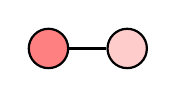
\begin{tikzpicture}[baseline=-0.1ex]
    \tikzset{tensor/.style = {minimum size = 0.5cm,shape = circle,thick,draw=black,inner sep = 0pt}, edge/.style = {thick,line width=.4mm},every loop/.style={}}
    \def\x{0}
    \def\y{0}
    \node[tensor,fill=red!50!white] (u) at (\x+1,\y) {$\ub$};
    \node[tensor,fill=red!20!white] (v) at (\x+2,\y) {$\vb$};
    \draw[edge] (u) -- (v);
    \end{tikzpicture}\right)}{\partial\left(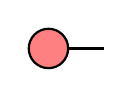
\begin{tikzpicture}[baseline=-0.1ex]
    \tikzset{tensor/.style = {minimum size = 0.5cm,shape = circle,thick,draw=black,inner sep = 0pt}, edge/.style = {thick,line width=.4mm},every loop/.style={}}
    \def\x{0}
    \def\y{0}
    \node[tensor,fill=red!50!white] (u) at (\x+1,\y) {$\ub$};
    \draw[edge] (u) -- (\x+1.7,\y);
    \end{tikzpicture}\right)}
=
    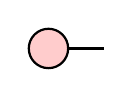
\begin{tikzpicture}[baseline=-0.1ex]
    \tikzset{tensor/.style = {minimum size = 0.5cm,shape = circle,thick,draw=black,inner sep = 0pt}, edge/.style = {thick,line width=.4mm},every loop/.style={}}
    \def\x{6}
    \def\y{0}
    \node[tensor,fill=red!20!white] (v) at (\x+2,\y) {$\vb$};
    \draw[edge] (v) -- (\x+2.7,\y);
    \end{tikzpicture}
    =
    \vb
    $
\item
    $\frac{\partial\Ab\xb}{\partial\xb}
=
    \frac{\partial\left(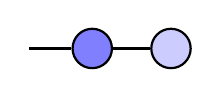
\begin{tikzpicture}[baseline=-0.1ex]
    \tikzset{tensor/.style = {minimum size = 0.5cm,shape = circle,thick,draw=black,inner sep = 0pt}, edge/.style = {thick,line width=.4mm},every loop/.style={}}
    \def\x{6}
    \def\y{0}
    \node[tensor,fill=blue!50!white] (A) at (\x+1,\y) {$\Ab$};
    \node[tensor,fill=blue!20!white] (x) at (\x+2,\y) {$\xb$};
    \draw[edge] (A) -- (x);
    \draw[edge] (A) -- (\x+0.2,\y);
    \end{tikzpicture}\right)}{\partial\left(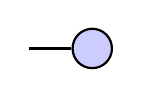
\begin{tikzpicture}[baseline=-0.1ex]
    \tikzset{tensor/.style = {minimum size = 0.5cm,shape = circle,thick,draw=black,inner sep = 0pt}, edge/.style = {thick,line width=.4mm},every loop/.style={}}
    \def\x{6}
    \def\y{0}
    \node[tensor,fill=blue!20!white] (x) at (\x+1,\y) {$\xb$};
    \draw[edge] (x) -- (\x+0.2,\y);
    \end{tikzpicture}\right)}
=
    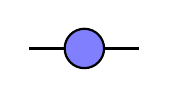
\begin{tikzpicture}[baseline=-0.1ex]
    \tikzset{tensor/.style = {minimum size = 0.5cm,shape = circle,thick,draw=black,inner sep = 0pt}, edge/.style = {thick,line width=.4mm},every loop/.style={}}
    \def\x{6}
    \def\y{0}
    \node[tensor,fill=blue!50!white] (A) at (\x+1,\y) {$\Ab$};
    \draw[edge] (A) -- (\x+0.3,\y);
    \draw[edge] (A) -- (\x+1.7,\y);
    \end{tikzpicture}
=
    \Ab
    $
    
\item 
    $\frac{\partial \xb^\ts\Ab\xb}{\partial\Ab}
=
    \frac{\partial\left(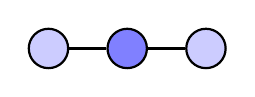
\begin{tikzpicture}[baseline=-0.1ex]
    \tikzset{tensor/.style = {minimum size = 0.5cm,shape = circle,thick,draw=black,inner sep = 0pt}, edge/.style = {thick,line width=.4mm},every loop/.style={}}
    \def\x{6}
    \def\y{0}
    \node[tensor,fill=blue!50!white] (A) at (\x+1,\y) {$\Ab$};
    \node[tensor,fill=blue!20!white] (x) at (\x+2,\y) {$\xb$};
    \node[tensor,fill=blue!20!white] (xt) at (\x,\y) {$\xb$};
    \draw[edge] (A) -- (x);
    \draw[edge] (A) -- (xt);
    \end{tikzpicture}\right)}{\partial\left(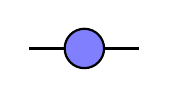
\begin{tikzpicture}[baseline=-0.1ex]
    \tikzset{tensor/.style = {minimum size = 0.5cm,shape = circle,thick,draw=black,inner sep = 0pt}, edge/.style = {thick,line width=.4mm},every loop/.style={}}
    \def\x{6}
    \def\y{0}
    \node[tensor,fill=blue!50!white] (A) at (\x+1,\y) {$\Ab$};
    \draw[edge] (A) -- (\x+1.7,\y);
    \draw[edge] (A) -- (\x+0.3,\y);
    \end{tikzpicture}\right)}
=
    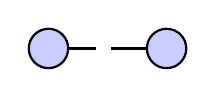
\begin{tikzpicture}[baseline=-0.1ex]
    \tikzset{tensor/.style = {minimum size = 0.5cm,shape = circle,thick,draw=black,inner sep = 0pt}, edge/.style = {thick,line width=.4mm},every loop/.style={}}
    \def\x{6}
    \def\y{0}
    \node[tensor,fill=blue!20!white] (x) at (\x+1,\y) {$\xb$};
    \node[tensor,fill=blue!20!white] (xt) at (\x-0.5,\y) {$\xb$};
    \draw[edge] (x) -- (\x+0.3,\y);
    \draw[edge] (xt) -- (\x+0.1,\y);
    \end{tikzpicture}
=
    \xb\outprod\xb
$
\item 
    $\frac{\partial\tr(\Ab)}{\partial\Ab}
    =
    \frac{\partial\left(
\begin{tikzpicture}[baseline=-0.1ex]
    \tikzset{tensor/.style = {minimum size = 0.5cm,shape = circle,thick,draw=black,inner sep = 0pt}, edge/.style = {thick,line width=.4mm},every loop/.style={}}
    \def\x{6}
    \def\y{0}
    \node[tensor,fill=blue!50!white] (A) at (\x+1,\y) {$\Ab$};
    \draw[edge] (A) to [out=20,in=160, distance=1cm] (A);
    \end{tikzpicture}\right)}
    {\partial\left(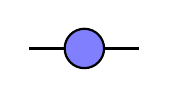
\begin{tikzpicture}[baseline=-0.1ex]
    \tikzset{tensor/.style = {minimum size = 0.5cm,shape = circle,thick,draw=black,inner sep = 0pt}, edge/.style = {thick,line width=.4mm},every loop/.style={}}
    \def\x{6}
    \def\y{0}
    \node[tensor,fill=blue!50!white] (A) at (\x+1,\y) {$\Ab$};
    \draw[edge] (A) -- (\x+1.7,\y);
    \draw[edge] (A) -- (\x+0.3,\y);
    \end{tikzpicture}\right)}
=

\begin{tikzpicture}[baseline=-0.1ex]
    \tikzset{tensor/.style = {minimum size = 0.5cm,shape = circle,thick,draw=black,inner sep = 0pt}, edge/.style = {thick,line width=.4mm},every loop/.style={}}
    \def\x{6}
    \def\y{0}
    \node[draw=none] (A) at (\x+1,\y) {};
    \draw[edge] (A) to [out=20,in=160, distance=1cm] (A);
    \end{tikzpicture}
=
    \Ib
    $
    \item
    $\frac{\partial\Ab\xb}{\partial\Ab}
=
    \frac{\partial\left(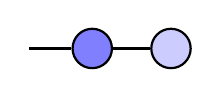
\begin{tikzpicture}[baseline=-0.1ex]
    \tikzset{tensor/.style = {minimum size = 0.5cm,shape = circle,thick,draw=black,inner sep = 0pt}, edge/.style = {thick,line width=.4mm},every loop/.style={}}
    \def\x{6}
    \def\y{0}
    \node[tensor,fill=blue!50!white] (A) at (\x+1,\y) {$\Ab$};
    \node[tensor,fill=blue!20!white] (x) at (\x+2,\y) {$\xb$};
    \draw[edge] (A) -- (x);
    \draw[edge] (A) -- (\x+0.2,\y);
    \end{tikzpicture}\right)}{\partial\left(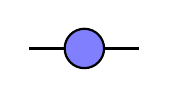
\begin{tikzpicture}[baseline=-0.1ex]
    \tikzset{tensor/.style = {minimum size = 0.5cm,shape = circle,thick,draw=black,inner sep = 0pt}, edge/.style = {thick,line width=.4mm},every loop/.style={}}
    \def\x{6}
    \def\y{0}
    \node[tensor,fill=blue!50!white] (A) at (\x+1,\y) {$\Ab$};
    \draw[edge] (A) -- (\x+0.3,\y);
    \draw[edge] (A) -- (\x+1.7,\y);
    \end{tikzpicture}\right)}
=
    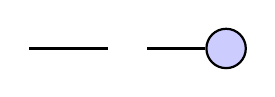
\begin{tikzpicture}[baseline=-0.1ex]
    \tikzset{tensor/.style = {minimum size = 0.5cm,shape = circle,thick,draw=black,inner sep = 0pt}, edge/.style = {thick,line width=.4mm},every loop/.style={}}
    \def\x{6}
    \def\y{0}
    \draw[edge] (\x+2,\y) -- (\x+3,\y);
    \node[tensor,fill=blue!20!white] (x) at (\x+4.5,\y) {$\xb$};
    \draw[edge] (x) -- (\x+3.5,\y);
    \node[draw=none] at (\x+3.25,\y){$\outprod$};
    \end{tikzpicture}
=
    \Ib\outprod\xb
$,
\end{enumerate}
where in the last identity, the result is a third-order tensor.
Theorem~\ref{thm:gradients} applies when the tensor with respect to which the derivative is taken appears only once in the network. The following theorem shows how to handle the case where the tensor appears multiple times.
\begin{theorem}\label{thm:multiple-tensors-gradients}
    Let $\Tt$ be a tensor network where $\Gt$ is a core tensor. If $\Gt$ appears $k$ times in the tensor network of $\Tt$, then $\frac{\partial\Tt}{\partial\Gt}$ is obtained by summing $k$ copies of the tensor network of $\Tt$, where a different occurrence of $\Gt$ is removed in each copy.
\end{theorem}
The following examples illustrate how Theorem~\ref{thm:multiple-tensors-gradients} can be applied.
\paragraph{Examples}
\begin{itemize}
    \item Let $\xb\in\RR^{d}$ and $\Ab\in\RR^{d\times d}$
    \begin{align*}
    \frac{\partial \xb^\ts\Ab\xb}{\partial\xb}
=
    \frac{\partial\left(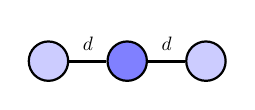
\begin{tikzpicture}[baseline=-0.1ex]
    \tikzset{tensor/.style = {minimum size = 0.5cm,shape = circle,thick,draw=black,inner sep = 0pt}, edge/.style = {thick,line width=.4mm},every loop/.style={}}
    \def\x{6}
    \def\y{0}
    \node[tensor,fill=blue!50!white] (A) at (\x+1,\y) {$\Ab$};
    \node[tensor,fill=blue!20!white] (x) at (\x+2,\y) {$\xb$};
    \node[tensor,fill=blue!20!white] (xprime) at 
    (\x,\y){$\xb$};
    \draw[edge] (A) -- (x)node [midway, above] {\scalebox{0.7}{\dimcolor{$d$}}};
    \draw[edge] (A) -- (xprime)node [midway, above] {\scalebox{0.7}{\dimcolor{$d$}}};
    \end{tikzpicture}\right)}{\partial\left(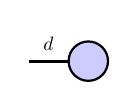
\begin{tikzpicture}[baseline=-0.1ex]
    \tikzset{tensor/.style = {minimum size = 0.5cm,shape = circle,thick,draw=black,inner sep = 0pt}, edge/.style = {thick,line width=.4mm},every loop/.style={}}
    \def\x{6}
    \def\y{0}
    \node[tensor,fill=blue!20!white] (x) at (\x,\y) {$\xb$};
    \draw[edge] (x) -- (\x-0.75,\y)node [midway, above] {\scalebox{0.7}{\dimcolor{$d$}}};
    \end{tikzpicture}\right)}
&=
    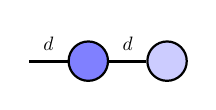
\begin{tikzpicture}[baseline=-0.1ex]
    \tikzset{tensor/.style = {minimum size = 0.5cm,shape = circle,thick,draw=black,inner sep = 0pt}, edge/.style = {thick,line width=.4mm},every loop/.style={}}
    \def\x{6}
    \def\y{0}
    \node[tensor,fill=blue!50!white] (A) at (\x+1,\y) {$\Ab$};
    \node[tensor,fill=blue!20!white] (x) at (\x+2,\y) {$\xb$};
    \draw[edge] (A) -- (x)node [midway, above] {\scalebox{0.7}{\dimcolor{$d$}}};
    \draw[edge] (A) -- (\x+0.25,\y)node [midway, above] {\scalebox{0.7}{\dimcolor{$d$}}};
    \end{tikzpicture}  
    +
    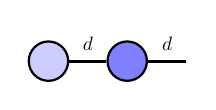
\begin{tikzpicture}[baseline=-0.1ex]
    \tikzset{tensor/.style = {minimum size = 0.5cm,shape = circle,thick,draw=black,inner sep = 0pt}, edge/.style = {thick,line width=.4mm},every loop/.style={}}
    \def\x{6}
    \def\y{0}
    \node[tensor,fill=blue!20!white] (x) at (\x+1,\y) {$\xb$};
    \node[tensor,fill=blue!50!white] (A) at (\x+2,\y) {$\Ab$};
    \draw[edge] (A) -- (x)node [midway, above] {\scalebox{0.7}{\dimcolor{$d$}}};
    \draw[edge] (A) -- (\x+2.75,\y)node [midway, above] {\scalebox{0.7}{\dimcolor{$d$}}};
    \end{tikzpicture}\\  
&=
    \Ab\xb + \Ab^\ts\xb = (\Ab\xb+\Ab^\ts)\xb.
\end{align*}
    \item 
Suppose $\Xb\in\RR^{n\times m},~\Wb\in\RR^{m\times n}$
    \begin{align*}
    \frac{\partial\norm{\Xb\Wb - \Yb}^2_F}{\partial \Wb}
&= 
    \frac{\partial\tr(\Wb^\ts\Xb^\ts\Xb\Wb)}{\partial\Wb}\\
&= 
    \frac{\partial\left( 
\begin{tikzpicture}[baseline=-0.1ex]
    \tikzset{tensor/.style = {minimum size = 0.5cm,shape = circle,thick,draw=black,inner sep = 0pt}, edge/.style = {thick,line width=.4mm},every loop/.style={}}
    \def\x{6}
    \def\y{0}
    \node[tensor,fill=red!20!white] (Wt) at (\x+1,\y) {$\Wb$};
    \node[tensor,fill=red!50!white] (Xt) at (\x+2,\y) {$\Xb$};
    \node[tensor,fill=red!50!white] (X) at (\x+3,\y) {$\Xb$};
    \node[tensor,fill=red!20!white] (W) at (\x+4,\y) {$\Wb$};
    \draw[edge] (Wt) -- (Xt)node [midway, above] {\scalebox{0.7}{\dimcolor{$m$}}};
    \draw[edge] (Xt) -- (X)node [midway, above] {\scalebox{0.7}{\dimcolor{$n$}}};
    \draw[edge] (X) -- (W)node [midway, above] {\scalebox{0.7}{\dimcolor{$n$}}};
    \draw[edge] (Wt) to [out=145,in=35, distance=1cm] (W);
    \end{tikzpicture}\right)}{\partial\left(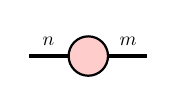
\begin{tikzpicture}[baseline=-0.1ex]
    \tikzset{tensor/.style = {minimum size = 0.5cm,shape = circle,thick,draw=black,inner sep = 0pt}, edge/.style = {thick,line width=.4mm},every loop/.style={}}
    \def\x{6}
    \def\y{0}   
    \node[tensor,fill=red!20!white] (W) at (\x+4,\y) {$\Wb$};
    \draw[edge] (W) -- (\x+4.75,\y)node [midway, above] {\scalebox{0.7}{\dimcolor{$m$}}};
    \draw[edge] (W) -- (\x+3.25,\y)node [midway, above] {\scalebox{0.7}{\dimcolor{$n$}}};
    \end{tikzpicture}\right)}\\
&=
    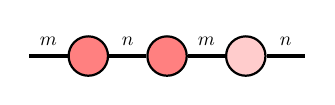
\begin{tikzpicture}[baseline=-0.1ex]
    \tikzset{tensor/.style = {minimum size = 0.5cm,shape = circle,thick,draw=black,inner sep = 0pt}, edge/.style = {thick,line width=.4mm},every loop/.style={}}
    \def\x{6}
    \def\y{0}
    \node[tensor,fill=red!50!white] (Xt) at (\x+2,\y) {$\Xb$};
    \node[tensor,fill=red!50!white] (X) at (\x+3,\y) {$\Xb$};
    \node[tensor,fill=red!20!white] (W) at (\x+4,\y) {$\Wb$};
    \draw[edge] (Xt) -- (\x+1.25,\y)node [midway, above] {\scalebox{0.7}{\dimcolor{$m$}}};
    \draw[edge] (Xt) -- (X)node [midway, above] {\scalebox{0.7}{\dimcolor{$n$}}};
    \draw[edge] (X) -- (W)node [midway, above] {\scalebox{0.7}{\dimcolor{$m$}}};
    \draw[edge] (W) -- (\x+4.75,\y)node [midway, above] {\scalebox{0.7}{\dimcolor{$n$}}};
    \end{tikzpicture}
+
    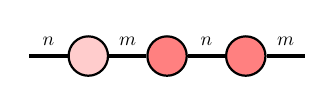
\begin{tikzpicture}[baseline=-0.1ex]
    \tikzset{tensor/.style = {minimum size = 0.5cm,shape = circle,thick,draw=black,inner sep = 0pt}, edge/.style = {thick,line width=.4mm},every loop/.style={}}
    \def\x{6}
    \def\y{0}
    \node[tensor,fill=red!20!white] (Wt) at (\x+1,\y) {$\Wb$};
    \node[tensor,fill=red!50!white] (Xt) at (\x+2,\y) {$\Xb$};
    \node[tensor,fill=red!50!white] (X) at (\x+3,\y) {$\Xb$};
    \draw[edge] (Wt) -- (Xt)node [midway, above] {\scalebox{0.7}{\dimcolor{$m$}}};
    \draw[edge] (Xt) -- (X)node [midway, above] {\scalebox{0.7}{\dimcolor{$n$}}};
    \draw[edge] (Wt) -- (\x+0.25,\y)node [midway, above] {\scalebox{0.7}{\dimcolor{$n$}}};
    \draw[edge] (X) -- (\x+3.75,\y)node [midway, above] {\scalebox{0.7}{\dimcolor{$m$}}};    
    \end{tikzpicture}\\
&=
2\Xb^\ts\Xb\Wb.
\end{align*}
\end{itemize}
We conclude this chapter by presenting several applications of tensor network gradients.
\subsection{Applications}
There is a wide range of applications for tensor network gradients, we highlight two notable examples here. 

We first briefly introduce the notion of loss functions and explain how the chain rule can be easily applied with expressions involving tensors and Jacobian tensors. A loss function $L:S\times S\to \RR^{\geq 0}$ serves to measure the error or cost incurred by a computational model, algorithm, or decision process when producing the output $\hat{y}\in S$ as a prediction of the ground truth $y\in S$. The goal of many learning and optimization algorithms is to minimize this loss. One approach is to use the Frobenius norm for the difference between the predicted output and the ground truth. To minimize the Frobenius norm when both the input and output are tensors, Jacobians can be used to compute the necessary gradients. Let $\At\in\RR^{d_1\times d_2\times d_3}$ be the ground truth and $\Tt\in\RR^{d_1\times d_2\times d_3}$ be the predicted output. Using Theorem~\ref{thm:gradients}, the gradient of the loss $L = \norm{\At-\Tt}_F^2$ can be written as:
    \begin{align*}
        \frac{\partial\norm{\At-\Tt}_F^2}{\partial\Tt} 
        &=
        \frac{\partial}{\partial\Tt}\left(\norm{\At}_F^2 + \norm{\Tt}_F^2 - 2\langle\At,\Tt\rangle\right)\\
        &= 
    \frac{\partial}{\partial\Tt}\left(\begin{tikzpicture}[baseline=\baseline]
    \tikzset{tensor/.style = {minimum size = 0.5cm,shape = circle,thick,draw=black,inner sep = 0pt}, edge/.style = {thick,line width=.4mm},every loop/.style={}}
    \def\y{0}
    \def\x{0}
    \node[tensor,fill=green!50!red!50!white] (St) at (\x,\y){\scalebox{0.85}{$\Tt$}};
    \node[tensor,fill=green!50!red!50!white] (Tt) at (\x+1,\y){\scalebox{0.85}{$\Tt$}};
    \draw[edge] (St) -- (Tt);
    \draw[edge] (St) to [out=45,in=135] (Tt);
    \draw[edge] (St) to [out=-45,in=-135] (Tt);
    \node[draw=none] () at (\x+0.5,\y+0.5) {\scalebox{0.7}{\dimcolor{$d_1$}}};
    \node[draw=none] () at (\x+0.5,\y+0.15) {\scalebox{0.7}{\dimcolor{$d_2$}}};
    \node[draw=none] () at (\x+0.5,\y-0.5) {\scalebox{0.7}{\dimcolor{$d_3$}}};
\end{tikzpicture}
-2
~
\begin{tikzpicture}[baseline=\baseline]
    \tikzset{tensor/.style = {minimum size = 0.5cm,shape = circle,thick,draw=black,inner sep = 0pt}, edge/.style = {thick,line width=.4mm},every loop/.style={}}
    \def\y{0}
    \def\x{0}
    \node[tensor,fill=blue!40!red!20!white] (St) at (\x,\y){\scalebox{0.85}{$\At$}};
    \node[tensor,fill=green!50!red!50!white] (Tt) at (\x+1,\y){\scalebox{0.85}{$\Tt$}};
    \draw[edge] (St) -- (Tt);
    \draw[edge] (St) to [out=45,in=135] (Tt);
    \draw[edge] (St) to [out=-45,in=-135] (Tt);
    \node[draw=none] () at (\x+0.5,\y+0.5) {\scalebox{0.7}{\dimcolor{$d_1$}}};
    \node[draw=none] () at (\x+0.5,\y+0.15) {\scalebox{0.7}{\dimcolor{$d_2$}}};
    \node[draw=none] () at (\x+0.5,\y-0.5) {\scalebox{0.7}{\dimcolor{$d_3$}}};
\end{tikzpicture}
\right)\\
&=
\left(\begin{tikzpicture}[baseline=\baseline]
    \tikzset{tensor/.style = {minimum size = 0.5cm,shape = circle,thick,draw=black,inner sep = 0pt}, edge/.style = {thick,line width=.4mm},every loop/.style={}}
    \def\y{0}
    \def\x{0}
    \node[tensor,fill=green!50!red!50!white] (Tt) at (\x,\y){\scalebox{0.85}{$\Tt$}};
    \draw[edge](Tt) -- (\x+0.85,\y)node[midway, above]{\edgelabel{$d_2$}};
    \draw[edge](Tt) -- (\x-0.85,\y)node[midway, above]{\edgelabel{$d_1$}};
    \draw[edge](Tt) -- (\x,\y-0.85)node[midway, left]{\edgelabel{$d_3$}};
    \end{tikzpicture}
+
\begin{tikzpicture}[baseline=\baseline]
    \tikzset{tensor/.style = {minimum size = 0.5cm,shape = circle,thick,draw=black,inner sep = 0pt}, edge/.style = {thick,line width=.4mm},every loop/.style={}}
    \def\y{0}
    \def\x{0}
    \node[tensor,fill=green!50!red!50!white] (Tt) at (\x,\y){\scalebox{0.85}{$\Tt$}};
    \draw[edge](Tt) -- (\x+0.85,\y)node[midway, above]{\edgelabel{$d_2$}};
    \draw[edge](Tt) -- (\x-0.85,\y)node[midway, above]{\edgelabel{$d_1$}};
    \draw[edge](Tt) -- (\x,\y-0.85)node[midway, left]{\edgelabel{$d_3$}};
    \end{tikzpicture}
-2~~
\begin{tikzpicture}[baseline=\baseline]
    \tikzset{tensor/.style = {minimum size = 0.5cm,shape = circle,thick,draw=black,inner sep = 0pt}, edge/.style = {thick,line width=.4mm},every loop/.style={}}
    \def\y{0}
    \def\x{0}
    \node[tensor,fill=blue!40!red!20!white] (Tt) at (\x,\y){\scalebox{0.85}{$\At$}};
    \draw[edge](Tt) -- (\x+0.85,\y)node[midway, above]{\edgelabel{$d_2$}};
    \draw[edge](Tt) -- (\x-0.85,\y)node[midway, above]{\edgelabel{$d_1$}};
    \draw[edge](Tt) -- (\x,\y-0.85)node[midway, left]{\edgelabel{$d_3$}};
    \end{tikzpicture}\right)\\
&=
2\left(\begin{tikzpicture}[baseline=\baseline]
    \tikzset{tensor/.style = {minimum size = 0.5cm,shape = circle,thick,draw=black,inner sep = 0pt}, edge/.style = {thick,line width=.4mm},every loop/.style={}}
    \def\y{0}
    \def\x{0}
    \node[tensor,fill=green!50!red!50!white] (Tt) at (\x,\y){\scalebox{0.85}{$\Tt$}};
    \draw[edge](Tt) -- (\x+0.85,\y)node[midway, above]{\edgelabel{$d_2$}};
    \draw[edge](Tt) -- (\x-0.85,\y)node[midway, above]{\edgelabel{$d_1$}};
    \draw[edge](Tt) -- (\x,\y-0.85)node[midway, left]{\edgelabel{$d_3$}};
    \end{tikzpicture}
-
\begin{tikzpicture}[baseline=\baseline]
    \tikzset{tensor/.style = {minimum size = 0.5cm,shape = circle,thick,draw=black,inner sep = 0pt}, edge/.style = {thick,line width=.4mm},every loop/.style={}}
    \def\y{0}
    \def\x{0}
    \node[tensor,fill=blue!40!red!20!white] (Tt) at (\x,\y){\scalebox{0.85}{$\At$}};
    \draw[edge](Tt) -- (\x+0.85,\y)node[midway, above]{\edgelabel{$d_2$}};
    \draw[edge](Tt) -- (\x-0.85,\y)node[midway, above]{\edgelabel{$d_1$}};
    \draw[edge](Tt) -- (\x,\y-0.85)node[midway, left]{\edgelabel{$d_3$}};
    \end{tikzpicture}\right).
\end{align*}
The chain rule can be easily extended to expressions involving tensor variables. Consider, for example, an arbitrary loss function $\mathcal{ L}: \mathbb{R}^{d_1\times \cdots \times d_N} \to \mathbb{R}$ that one wishes to minimize over the $N$-th order tensor inputs $\Tt$. Now suppose that the tensor input is parameterized as a tensor network where $\Gt \in \mathbb{R}^{m_1\times \cdots \times m_M}$ is an $M$-th order core tensor. To compute the Jacobian tensor of $\mathcal L$ with respect to $\Gt$, one can use the chain rule as follows: 
$$\frac{\partial  \mathcal L}{\partial\Gt} 
=
\frac{\partial \mathcal L}{\partial \Tt }\frac{\partial\Tt}{\partial\Gt}  $$
where $\frac{\partial  \mathcal L}{\partial\Gt}$ is of size $m_1\times\cdots \times m_M$, $\frac{\partial  \mathcal L}{\partial \Tt }$ is of size%
\footnote{One could say that,technically, $\frac{\partial  \mathcal L}{\partial\Gt}$ has shape $1\times m_1 \cdots \times m_M$  and $\frac{\partial  \mathcal L}{\partial \Tt }$ has shape $1\times d_1\times \cdots \times d_N$, but the first trivial mode of dimension $1$ is naturally omitted.}
$d_1\times \cdots \times d_N$, and $\frac{\partial\Tt}{\partial\Gt} $ is of size $d_1\times \cdots \times d_N \times m_1 \cdots \times m_M$. The product between $\frac{\partial  \mathcal L}{\partial \Tt }$ and $\frac{\partial\Tt}{\partial\Gt}  $ is implicitly understood as the contraction between the $M$ modes of $\frac{\partial  \mathcal L}{\partial \Tt }$ with the first $M$-modes  of $\frac{\partial\Tt}{\partial\Gt}  $.

We are now ready to conclude this chapter by presenting two applications of tensor network gradient computations. 
\begin{itemize}
\item\textbf{CP Decomposition with Gradient Descent} To find an approximate CP decomposition~(see Section~\ref{sec:cp-decomposition}) of a tensor $\Tt\in\RR^{d_1\times\cdots\times d_N}$, one can use gradient descent to minimize the loss $L = \norm{\Tt-\CP{\Gb_1,\cdots,\Gb_N}}^2_F$. Here $\CP{\Gb_1,\cdots,\Gb_N}$ denotes the CP decomposition where $\Gb_1,\cdots,\Gb_N$ are the factor matrices. To optimize w.r.t. the factor matrices, we can apply gradient descent to the loss function. For instance, in the case of $N=3$, to compute $\Gb_1$  we can apply the chain rule and write $\frac{\partial L}{\partial\Gb_1} = \frac{\partial L}{\partial\CP{\Gb_1,\Gb_2,\Gb_3}}\frac{\partial\CP{\Gb_1,\Gb_2,\Gb_3}}{\partial\Gb_1}$, where $\frac{\partial L}{\partial\CP{\Gb_1,\Gb_2,\Gb_3}}= 2(\Tt-\CP{\Gb_1,\Gb_2,\Gb_3})\in\RR^{d_1\times d_2\times d_3}$ and 
\begin{align*}
\frac{\partial\CP{\Gb_1,\Gb_2,\Gb_3}}{\partial\Gb_1}
=
\begin{tikzpicture}[baseline=\baseline]
    \tikzset{tensor/.style = {minimum size = 0.5cm,shape = circle,thick,draw=black,inner sep = 0pt}, edge/.style   = {thick,line width=.4mm},every loop/.style={}}
    \def\y{0}
    \def\x{0}
 \node[tensor,fill=blue!50!white] (G2) at (\x+1,\y){$\Gb_2$};
   \node[tensor,fill=blue!20!white] (G3) at (\x+2,\y){$\Gb_3$};
    \draw  node[fill = black,circle,inner sep=0pt,minimum size=4pt] (m) at (\x+1,\y+1) {};
    \draw[edge] (m) -- (\x,\y+0.1) node [midway,left] {\edgelabel{$R$}};
    \draw[edge] (G2) -- (m)node [midway,left] {\edgelabel{$R$}};
    \draw[edge] (G3) -- (m)node [midway,right] {\edgelabel{$R$}};
    \draw[edge](\x,\y-0.1) -- (\x,\y-0.7) node [midway,right] {\edgelabel{$d_1$}};
    \draw[edge](G2) -- (\x+1,\y-0.7)node [midway,left] {\edgelabel{$d_2$}};
    \draw[edge](G3) -- (\x+2,\y-0.7) node [midway,left] {\edgelabel{$d_3$}};
\end{tikzpicture}\in\RR^{d_1\times d_2\times d_3\times R}.
\end{align*}
Looking at the resulting TN, one can see that it can be expressed using matricizations and the Khatri-Rao product:
\begin{align*}
  \frac{\partial L}{\partial\Gb_1} 
&=
\frac{\partial L}{\partial\CP{\Gb_1,\Gb_2,\Gb_3}}\frac{\partial\CP{\Gb_1,\Gb_2,\Gb_3}}{\partial\Gb_1}\\
&=
\begin{tikzpicture}[baseline=-0.5ex]
    \tikzset{tensor1/.style = {minimum width = 3cm,minimum height = 0.6cm,shape = rounded rectangle,thick,draw=black,inner sep = 0pt}, edge/.style = {thick,line width=.4mm},every loop/.style={}}
     \tikzset{tensor2/.style = {minimum size = 0.5cm,shape = circle,thick,draw=black,inner sep = 0pt}, edge/.style   = {thick,line width=.4mm},every loop/.style={}}
    \def\y{1}
    \def\x{0}
    \node[tensor1,fill=blue!45!red!20!white] (Tt) at (\x,\y){$2(\Tt-\CP{\Gb_1,\Gb_2,\Gb_3})$};
    \node[tensor2,fill=blue!50!white] (G2) at (\x,\y-1){$\Gb_2$};
   \node[tensor2,fill=blue!20!white] (G3) at (\x+1,\y-1){$\Gb_3$};
    \draw  node[fill = black,circle,inner sep=0pt,minimum size=4pt] (m) at (\x+0.5,\y-1.85) {};
    \draw[edge](G2)--(m)node [midway,left] {\edgelabel{$R$}};
    \draw[edge](G3)--(m)node [midway,right] {\edgelabel{$R$}};    \draw[edge](Tt)--(G2)node [midway,left] {\edgelabel{$d_2$}};
    \draw[edge](\x+1,\y-0.3)--(G3)node [midway,left] {\edgelabel{$d_3$}};
    \draw[edge](m)--(\x+0.5,\y-2.25)node [midway,left] {\edgelabel{$R$}};
    \draw[edge](\x-0.75,\y-0.3) -- (\x-0.75,\y-2.25)node [midway,left] {\edgelabel{$d_1$}};
\end{tikzpicture}\\
&=\begin{tikzpicture}[baseline=-0.5ex]
    \tikzset{tensor/.style = {minimum width = 3cm,minimum height = 0.6cm,shape = rounded rectangle,thick,draw=black,inner sep = 0pt}, edge/.style = {thick,line width=.4mm},every loop/.style={}}
    \def\y{1}
    \def\x{0}
    \node[tensor,fill=blue!45!red!20!white] (Tt) at (\x,\y){$2(\Tt-\CP{\Gb_1,\Gb_2,\Gb_3})$};
    \node[tensor,fill=blue!25!red!45!white] (Gt) at (\x+1,\y-1){$\Gb_2\krao\Gb_3$};
    \draw[edge](\x+0.5,\y-0.3) -- (\x+0.5,\y-0.7);
    \draw[edge](\x+0.6,\y-0.3) -- (\x+0.6,\y-0.7)node [midway,right] {\edgelabel{$d_2d_3$}};
    \draw[edge](\x-0.75,\y-0.3) -- (\x-0.75,\y-2)node [midway,left] {\edgelabel{$d_1$}};
    \draw[edge](\x+0.85,\y-1.3) -- (\x+0.85,\y-2)node [midway,left] {\edgelabel{$R$}};
\end{tikzpicture}\\
&=
2(\Tt-\CP{\Gb_1,\Gb_2,\Gb_3})_{(1)}(\Gb_2\krao\Gb_3)
\in\RR^{d_1\times R}.
\end{align*}
 \item\textbf{Machine Learning} To compress neural networks, the dense weight matrices of fully connected layers can be parameterized using tensor factorizations to reduce memory usage~\citep{novikov2015tensorizing}. Let $\Wb\in\RR^{P\times D}$ be a weight matrix and $\xb\in\RR^{D}$ the input vector of a neural network layer. The output $\yb\in\RR^{P}$ is obtained by contracting the weight matrix $\Wb$ with the input vector $\xb$. 
    Suppose $P = \Pi_{i=1}^N{p_i}$ and $D =\Pi_{i=1}^Nd_i$. Then by reshaping $\Wb$ and $\xb$ in tensors we have
\begin{align*}
    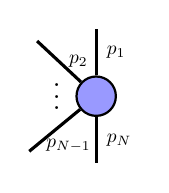
\begin{tikzpicture}[baseline=-0.1ex]
    \tikzset{tensor/.style = {minimum size = 0.5cm,shape = circle,thick,draw=black,inner sep = 0pt}, edge/.style = {thick,line width=.4mm},every loop/.style={}}
    \def\x{6}
    \def\y{0}
    \node[tensor,fill=blue!40!white] (y) at (\x,\y) {$\Yt$};
    \draw[edge](y)--(\x,\y+0.85)node [midway,right] {\scalebox{0.7}{\dimcolor{$p_1$}}};
    \draw[edge](y)--(\x-0.75,\y+0.7)node [midway,right=-0.01cm] {\scalebox{0.7}{\dimcolor{$p_2$}}};
    \draw[edge](y)--(\x-0.85,\y-0.7)node [very near end,right] {\scalebox{0.7}{\dimcolor{$p_{N-1}$}}};
    \draw[edge](y)--(\x,\y-0.85)node [midway,right] {\scalebox{0.7}{\dimcolor{$p_N$}}};
    \node[draw=none] at (\x-0.5,\y+0.1){$\vdots$};
    \end{tikzpicture}
=\sum_{d_1,\cdots,d_N}\Wt_{p_1,\cdots, p_N,d_1,\cdots, d_N}\Xt_{d_1,\cdots, d_N} =
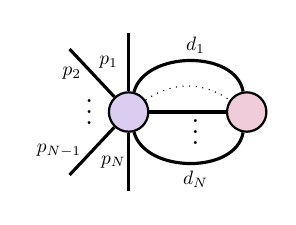
\begin{tikzpicture}[baseline=-0.1ex]
    \tikzset{tensor/.style = {minimum size = 0.5cm,shape = circle,thick,draw=black,inner sep = 0pt}, edge/.style = {thick,line width=.4mm},every loop/.style={}}
    \def\x{6}
    \def\y{0}
    \node[tensor,fill=red!30!blue!20!white] (w) at (\x,\y) {$\Wt$};
    \node[tensor,fill=blue!30!red!20!white] (x) at (\x+1.5,\y) {$\Xt$};
    \draw[edge](w)--(x);
    \draw[edge](w)--(\x,\y+1)node [midway,left] {\scalebox{0.7}{\dimcolor{$p_1$}}};
    \draw[edge](w)--(\x-0.75,\y+0.8)node [midway,left] {\scalebox{0.7}{\dimcolor{$p_2$}}};
    \draw[edge](w)--(\x-0.75,\y-0.8)node [midway,left] {\scalebox{0.7}{\dimcolor{$p_{N-1}$}}};
    \draw[edge](w)--(\x,\y-1)node [midway,left=-0.1cm] {\scalebox{0.7}{\dimcolor{$p_N$}}};
    \node[draw=none] at (\x-0.5,\y+0.1){$\vdots$};
   \draw[edge] (w) to [out=-75,in=-100] (x);
    \draw[edge] (w) to [out=75,in=100] (x);
    \draw[dotted] (w) to [out=35,in=145] (x);
    \node[draw=none] at (\x+0.85,\y-0.15){$\vdots$};
    \node[draw=none] () at (\x+0.85,\y+0.85) {\scalebox{0.7}{\dimcolor{$d_1$}}};
    (\x+1.2,\y-0.2){$\vdots$};
    \node[draw=none] () at (\x+0.85,\y-0.85) {\scalebox{0.7}{\dimcolor{$d_N$}}};
\end{tikzpicture}.
\end{align*}
For simplicity, we proceed with the case $N=4$. In~\citep{novikov2015tensorizing}, the authors propose to parameterize $\Wt$ in the MPO format~(see Section~\ref{sec:efficient-operations}). i.e., 
$\Wt = 
\begin{tikzpicture}[baseline=\baseline]
    \tikzset{tensor/.style = {minimum size = 0.5cm,shape = circle,thick,draw=black,inner sep = 0pt}, edge/.style   = {thick,line width=.4mm},every loop/.style={}}
    \def\y{0}
    \def\x{0}
  \node[tensor,fill=red!30!white] (G1) at (\x,\y){$\Gt_1$};
  \node[tensor,fill=red!50!white] (G2) at (\x+1,\y){\scalebox{0.85}{$\Gt_2$}};
  \node[tensor,fill=blue!30!white] (G3) at (\x+2,\y){$\Gt_3$};
  \node[tensor,fill=blue!50!white] (G4) at (\x+3,\y){$\Gt_4$};
    \draw[edge](G1) -- (\x,\y-0.85)node [midway,left] {\edgelabel{$d_1$}};
    \draw[edge](G2) -- (\x+1,\y-0.85)node [midway,left] {\edgelabel{$d_2$}};
     \draw[edge](G3) -- (\x+2,\y-0.85)node [midway,left] {\edgelabel{$d_3$}};
    \draw[edge](G4) -- (\x+3,\y-0.85)node [midway,left] {\edgelabel{$d_4$}};
    \draw[edge](G1) -- (G2) node [midway,above] {\edgelabel{$R_1$}};
    \draw[edge](G2) -- (G3) node [midway,above] {\edgelabel{$R_2$}};
    \draw[edge](G3) -- (G4) node [midway,above] {\edgelabel{$R_3$}};
    \draw[edge](G1) -- (\x,\y+0.85)node [midway,left] {\edgelabel{$p_1$}};
    \draw[edge](G2) -- (\x+1,\y+0.85)node [midway,left] {\edgelabel{$p_2$}};
    \draw[edge](G3) -- (\x+2,\y+0.85)node [midway,left] {\edgelabel{$p_3$}};
    \draw[edge](G4) -- (\x+3,\y+0.85)node [midway,left] {\edgelabel{$p_4$}};
\end{tikzpicture}.$
During the backpropagation step, since we aim to update the weight matrix, we need to optimize it with respect to all the core tensors. According to the chain rule, this gives: $\frac{\partial L}{\partial \Gt_i} = \frac{\partial L}{\partial \Yt}\frac{\partial\Yt}{\partial\Gt_i}$ for $i\in[4]$, where $L$ denotes the loss function. For instance, for $i=2$ we need to find the derivative of $\Yt$ with respect to $\Gt_2$. By applying Theorem~\ref{thm:gradients} we just need to remove $\Gt_2$ from the tensor network to obtain the result:
\begin{align*}
\frac{\partial\Yt}{\partial\Gt_2} 
&=
\frac{\partial\left(\begin{tikzpicture}[baseline=\baseline]
    \tikzset{tensor/.style = {minimum size = 0.5cm,shape = circle,thick,draw=black,inner sep = 0pt}, edge/.style   = {thick,line width=.4mm},every loop/.style={}}
    \def\y{0}
    \def\x{0}
  \node[tensor,fill=red!30!white] (G1) at (\x,\y){$\Gt_1$};
  \node[tensor,fill=red!50!white] (G2) at (\x+1,\y){\scalebox{0.85}{$\Gt_2$}};
  \node[tensor,fill=blue!30!white] (G3) at (\x+2,\y){$\Gt_3$};
  \node[tensor,fill=blue!50!white] (G4) at (\x+3,\y){$\Gt_4$};
  \node[tensor,fill=blue!30!red!20!white] (x) at (\x+1.5,\y-1.5) {$\Xt$};
    \draw[edge](G1) -- (\x,\y-0.85)node [midway,left] {\edgelabel{$d_1$}};
    \draw[edge](x)--(\x,\y-0.85);
    \draw[edge](G2) -- (\x+1,\y-0.85)node [midway,left] {\edgelabel{$d_2$}};
    \draw[edge](x)--(\x+1,\y-0.85);
     \draw[edge](G3) -- (\x+2,\y-0.85)node [midway,left] {\edgelabel{$d_3$}};
    \draw[edge](x)--(\x+2,\y-0.85);
    \draw[edge](G4) -- (\x+3,\y-0.85)node [midway,left] {\edgelabel{$d_4$}};
    \draw[edge](x)--(\x+3,\y-0.85);
    \draw[edge](G1) -- (G2) node [midway,above] {\edgelabel{$R_1$}};
    \draw[edge](G2) -- (G3) node [midway,above] {\edgelabel{$R_2$}};
    \draw[edge](G3) -- (G4) node [midway,above] {\edgelabel{$R_3$}};
    \draw[edge](G1) -- (\x,\y+0.85)node [midway,left] {\edgelabel{$p_1$}};
    \draw[edge](G2) -- (\x+1,\y+0.85)node [midway,left] {\edgelabel{$p_2$}};
    \draw[edge](G3) -- (\x+2,\y+0.85)node [midway,left] {\edgelabel{$p_3$}};
    \draw[edge](G4) -- (\x+3,\y+0.85)node [midway,left] {\edgelabel{$p_4$}};
\end{tikzpicture}\right)}{\partial\Gt_2}\\
&=
\begin{tikzpicture}[baseline=\baseline]
    \tikzset{tensor/.style = {minimum size = 0.5cm,shape = circle,thick,draw=black,inner sep = 0pt}, edge/.style   = {thick,line width=.4mm},every loop/.style={}}
    \def\y{-1}
    \def\x{0}
  \node[tensor,fill=red!30!white] (G1) at (\x,\y+1.5){$\Gt_1$};
    \node[tensor,fill=blue!30!white] (G3) at (\x+2,\y+1.5){$\Gt_3$};
  \node[tensor,fill=blue!50!white] (G4) at (\x+3,\y+1.5){$\Gt_4$};
  \node[tensor,fill=blue!30!red!20!white] (x) at (\x+1.5,\y) {$\Xt$};
    \draw[edge](G1) -- (\x,\y+0.85)node [midway,left] {\edgelabel{$d_1$}};
    \draw[edge](x)--(\x,\y+0.85);
    \draw[edge](\x+1,\y+1.35) -- (\x+1,\y+0.85)node [midway,left] {\edgelabel{$d_2$}};
    \draw[edge](x)--(\x+1,\y+0.85);
     \draw[edge](G3) -- (\x+2,\y+0.85)node [midway,left] {\edgelabel{$d_3$}};
    \draw[edge](x)--(\x+2,\y+0.85);
    \draw[edge](G4) -- (\x+3,\y+0.85)node [midway,left] {\edgelabel{$d_4$}};
    \draw[edge](x)--(\x+3,\y+0.85);
    \draw[edge](G3) -- (G4) node [midway,above] {\edgelabel{$R_3$}};
    \draw[edge](G1) -- (\x,\y+2.35)node [midway,left] {\edgelabel{$p_1$}};
    \draw[edge](G3) -- (\x+2,\y+2.35)node [midway,left] {\edgelabel{$p_3$}};
    \draw[edge](G4) -- (\x+3,\y+2.35)node [midway,left] {\edgelabel{$p_4$}};
    \draw[edge](G1)--(\x+0.85,\y+1.5) node [midway,above] {\edgelabel{$R_1$}};
    \draw[edge](G3)--(\x+1.25,\y+1.5) node [midway,above] {\edgelabel{$R_2$}};
    \draw[edge](\x+1,\y+1.6)--(\x+1,\y+2.35) node [midway,left] {\edgelabel{$p_2$}};
\end{tikzpicture}\in\RR^{p_1\times R_1\times p_2\times R_2\times p_3\times p_4\times d_2}.
\end{align*}
The gradient of the loss is thus given by
\begin{align*}
    \frac{\partial L}{\partial\Gt_2} = \frac{\partial L}{\partial\Yt}\frac{\partial \Yt}{\partial\Gt_2}
    =
    \begin{tikzpicture}[baseline=\baseline]
    \tikzset{tensor/.style = {minimum size = 0.5cm,shape = circle,thick,draw=black,inner sep = 0pt}, edge/.style   = {thick,line width=.4mm},every loop/.style={}}
    \def\y{-1.5}
    \def\x{0}
    \node[tensor,fill=green!30!white] (L) at (\x+1.5,\y+3.25){$\frac{\partial L}{\partial\Yt}$};
  \node[tensor,fill=red!30!white] (G1) at (\x,\y+1.5){$\Gt_1$};
    \node[tensor,fill=blue!30!white] (G3) at (\x+2,\y+1.5){$\Gt_3$};
  \node[tensor,fill=blue!50!white] (G4) at (\x+3,\y+1.5){$\Gt_4$};
  \node[tensor,fill=blue!30!red!20!white] (x) at (\x+1.5,\y) {$\Xt$};
    \draw[edge](G1) -- (\x,\y+0.85)node [midway,left] {\edgelabel{$d_1$}};
    \draw[edge](x)--(\x,\y+0.85);
    \draw[edge](\x+1,\y+1.35) -- (\x+1,\y+0.85)node [midway,left] {\edgelabel{$d_2$}};
    \draw[edge](x)--(\x+1,\y+0.85);
     \draw[edge](G3) -- (\x+2,\y+0.85)node [midway,left] {\edgelabel{$d_3$}};
    \draw[edge](x)--(\x+2,\y+0.85);
    \draw[edge](G4) -- (\x+3,\y+0.85)node [midway,left] {\edgelabel{$d_4$}};
    \draw[edge](x)--(\x+3,\y+0.85);
    \draw[edge](G3) -- (G4) node [midway,above] {\edgelabel{$R_3$}};
    \draw[edge](G1) -- (\x,\y+2.35)node [midway,left] {\edgelabel{$p_1$}};
    \draw[edge](L)--(\x,\y+2.35);
    \draw[edge](G3) -- (\x+2,\y+2.35)node [midway,left] {\edgelabel{$p_3$}};
    \draw[edge](L)--(\x+2,\y+2.35);
    \draw[edge](G4) -- (\x+3,\y+2.35)node [midway,left] {\edgelabel{$p_4$}};
    \draw[edge](L)--(\x+3,\y+2.35);
    \draw[edge](G1)--(\x+0.85,\y+1.5) node [midway,above] {\edgelabel{$R_1$}};
    \draw[edge](G3)--(\x+1.25,\y+1.5) node [midway,above] {\edgelabel{$R_2$}};
    \draw[edge](\x+1,\y+1.6)--(\x+1,\y+2.35) 
    node [midway,left] {\edgelabel{$p_2$}};
    \draw[edge](L)--(\x+1,\y+2.35);
\end{tikzpicture}\in\RR^{R_1\times p_2\times R_2\times d_2}.
\end{align*}

\end{itemize}






